\section{The model}
In this section, we explore foundational concepts in functional analysis and refine the definition of the gradient using the Riesz Representation Theorem. We then compute the gradient of the empirical loss functional under the assumption that the hypothesis space is a Reproducing Kernel Hilbert Space (RKHS). Our analysis uncovers a bias in the gradient estimation step of Friedman's boosting algorithm. To rectify this bias, we propose using the vector, derived from evaluating the gradient function at sample points, as the negative gradient vector in our boosting algorithm.

The objective of a gradient-boosting machine is to pinpoint an element within the hypothesis space that minimizes the empirical loss function. This goal is typically achieved via a gradient descent algorithm that operates within a functional space. However, performing gradient descent in such a space requires the use of more advanced mathematical tools. Thus, we initiate this section by presenting the necessary preliminaries in functional analysis.



\subsection{Preliminaries}

To provide a more detailed description of our model, we first introduce some notions in functional analysis.
Let $\mathcal{H}$ be a vector space. We define the evaluation functional $E_x$ as the function that maps a functional in $\mathcal{H}$ to its function value at $x$. Specifically, let
\begin{equation}\label{eq:eval-functional}
E_x: \mathcal{H} \to \R, \quad f \mapsto f(x).
\end{equation}

Observe that $E_x(f+g) = (f+g)(x) = E_x(f) + E_x(g)$, which implies that $E_x$ is a linear functional on $\mathcal{H}$.

In Equation \ref{eq:eval-functional}, we use the notation $\mathcal{H}$ to represent a function space because $\mathcal{H}$ often stands for the hypothesis space or the Hilbert space. A Hilbert space is a complete inner product space. The norm measures the distance between vectors, while the inner product can describe the correlation between two elements in a space. Since we need to discuss certain analytic properties, such as continuity, differentiability, or general limits, we require a complete space in which every Cauchy sequence has a limit. This is where a Hilbert space comes into play. It combines the aforementioned requirements and is thus widely used in this context.

Another crucial concept is the Frechet derivative. The Frechet derivative is a method to extend the derivative to function spaces. It measures the rate of change of a functional under small perturbations of its arguments. The Fréchet derivative is defined as the best linear approximation of the functional at a given point. Specifically, we define the Fréchet derivative of $f$ as a map from $\mathcal{X}$ to a linear functional $D_{f,x}$ on $\mathcal{X}$,
$$
D_{f}: \mathrm{int}_{\mathcal{X}} \to B(\mathcal{X},\mathcal{Y}), \quad x \mapsto D_{f,x}.
$$
To get an insight into $D_f$, we take a multivariate function as an example. In calculus, we have that. 
$$
D_{f,x_0} = \sum_{i=1}^n \partial f_i (x_o) \D x_i.
$$
%\begin{Example}
%Suppose $f: \R^n \to \R$, the frechet deritive of $f$ at $x_0$ is 
%
%\begin{eqnarray*}
%D_{f,x_0} &=& \sum_{i=1}^n \partial_i f (x_0) \D x_i \\
%&=& \mathbf{J}_f^x \D \x
%\end{eqnarray*}
%\end{Example}
Where
$$
\D x_i : \R^n \to \R, \quad h \mapsto h_i.
$$
Note that $\D x_i$ is the dual bases on $\R^n$ with respect to standard normal basis, since
$$
\D x_i (e_j) = \delta_{ij}.
$$

%\begin{Example}
%Suppose $f: \R^n \to \R^m$, then the frechet of $f$ at $x_0$ is 
%\end{Example}

%
%\begin{Proposition}[Rules of differentiation] \ \\
%\begin{itemize}
%	\item $D_{af,x} = a D_{f,x}.$
%	\item $D_{f+g,x} = D_{f,x} + D_{g,x}$
%	\item $D_{fg,x} = g(x)D_{f,x} + f(x)D_{g,x}$
%\end{itemize}
%\end{Proposition}
%
%\begin{Proposition}[The Chain Rule] \ \\
%Let X,Y and Z be normed vector spaces. Let $f: X \to Y$ and $g: Y \to Z$ are two maps such that $f$ is frechet differentiable at $x \in \mathrm{int}_X$ and $g$ at $f(x) \in \mathrm{int}_Y.$ Then, $g \circ f$ is frechet differentiable at $x$, and
%\begin{equation}\label{thm:ChainRule}
%	D_{g \circ f},x = D_{g,f(x)} \circ D_{f,x}
%\end{equation}
%\end{Proposition}
%\begin{proof}
%$$
%f(\omega+x) - f(x) = D_{f,x}(w) + \E_{f,x}(\omega)
%$$
%
%In addition,
%$$
%g(\omega+f(x))- g(f(x)) = D_{g,f(x)}(\omega) + \E_{g,f(x)}(\omega).
%$$
%thus
%
%\begin{eqnarray*}
%g(f(\omega+x))-g(f(x)) &=& D_{g,f(x)}(f(\omega+x)-f(x)) + \E_{g,f(x)}(f(\omega)) \\
%&=& D_{g,f(x)}( D_{f,x}(\omega)) + D_{g,f(x)}(\E_{f,x}(\omega)) + \E_{g,f(x)} \\
%&=& (D_{g,f(x)} \circ D_{f,x})(\omega) + \E_{g\circ f,x}(\omega).                                                                                                                                                                                                                                                                                                                                                                                                                  
%\end{eqnarray*}
%
%\end{proof}


%\begin{Proposition}[Differentiation of inverse function] \ \\
%Suppose $V$ is normed vector space and $f: V \to V$. Then
%$$
%D_{f^{-1},x} = (D_{f,f^{-1}(x)})^{-1} \circ D_{I,x},
%$$
%where 
%$$
%(D_{f,f^{-1}(x)})^{-1}(a) = (\mathrm{J}_f^{f^{-1}(x)})^{-1} a.
%$$
%\end{Proposition}



Next, we will introduce a widely used theorem for understanding function spaces' structure. This theorem has many applications in mathematics, physics, and even economics. For example, the Riesz representation theorem in finance implies that a payoff can represent any linear functional on the asset span.

\begin{Theorem}[Riesz Representation Theorem] \ \\ 
Suppose $\varphi$ is a bounded linear functional on a Hilbert space $V$. Then there exists a unique $h \in V$ such that
$$
\varphi(f) = \inner{f}{h}, \quad f \in \mathcal{H}.
$$
\end{Theorem}
The Riesz Representation Theorem is a cornerstone in functional analysis, establishing a one-to-one correspondence between linear functionals on a Hilbert space and the elements within that space. Specifically, it stipulates that for any bounded linear functional $f$ on a Hilbert space $\mathcal{H}$, there exists a unique element $h$ in $\mathcal{H}$ such that $\varphi(f) = \langle f, h\rangle$ for all $f$ in $\mathcal{H}$. Here, $\langle\cdot,\cdot\rangle$ denotes the inner product on $\mathcal{H}$.

In a complete normed vector space, the continuity of a linear functional is equivalent to its boundedness. Given the essential role of the evaluation functional in our model, we require a more suitable space to explore it. It's important to note that not all evaluation functionals of a Hilbert space are bounded. To satisfy the Riesz Representation Theorem's requirements, we define the Reproducing Kernel Hilbert Space (RKHS) as a space wherein every evaluation function is bounded, even though they may not consistently be so.

\begin{Definition}[RKHS] \ \\
	Let $X$ be a set and $\mathcal{H}$ a Hilbert space with $\mathcal{H} \subset \R^{X}$. If the evaluation functional $E_x$ over $\mathcal{H}$ is bounded. (or equivalently, continuous), then we say $\mathcal{H}$ is a Reproducing Kernel Hilbert Space.
\end{Definition}

Since the evaluation functional on $\mathcal{H}$ is bounded, the Riesz Representation Theorem suggests that there exists a unique vector $K_x \in \mathcal{H}$ which satisfies the following  
$$
f(x) = E_x(f) = \inner{f}{K_x}_{\mathcal{H}}.
$$
Also 
$$
K_x(y) = E_y(K_x) = \inner{K_x}{K_y}_{\mathcal{H}}.
$$
This allows us to define the reproducing kernel of $\mathcal{H}$ as a function. 
$$
K: X \times X \to \R, \quad (x,y) \mapsto K(x,y) = \inner{K_x}{K_y}_{\mathcal{H}}.
$$
\C{}
However, in practical applications, confirming whether the evaluation functional in a Hilbert space is bounded can be challenging. Even if it is bounded, the Riesz representation theorem only informs us of the existence of a kernel but does not give the analytic expression of the kernel. As a result, we commonly rely on a symmetric and positive definite function to construct a Hilbert space, known as the Moore-Aronszajn theorem.

\begin{Theorem}[Moore-Aronszajn] \ \\
Suppose $K$ is a symmetric positive definitive function on $X \times X$. Then there is a unique Hilbert Space of functions on $X$ for which $K$ is a reproducing Kernel.
	
\end{Theorem}

Next, we will give a better definition of the gradient. First, recall the definition of the gradient in calculus. It is a vector that points in the direction of the steepest increase of the function at a particular point. It can be calculated by taking the partial derivative with respect to each coordinate. The inner product of a gradient and the increment can be viewed as the linear approximation of the increment of the function value. This idea can be directly extended to a function space. Specifically, suppose $\MCH$ is a normed vector space, and $L$ is a function defined at $x_0 \in \MCH$. We know that $L$ is Frechet differentiable on $\MCH$ if and only if 
\begin{equation} \label{frechet}
	L(x_0 + h) = L(x_0) + D_{L,x_0}(h) + e_{x_0}(h), \quad \forall h \in \mathcal{H}.
\end{equation}

Where $D_{L,x_0}$ is a linear functional on $\MCH$ and the error part must moves faster to zero than $h$, that is 
$$\lim_{h \to 0} \frac{e_{x_0} (h)}{\Vert h \Vert} = 0.$$
Note that the zero on the right side of the above equation is the additive identity($0: \mathcal{H} \to \R,\quad f \mapsto 0$) in $\mathcal{H}$ rather than the real number $0$.

Now, the Riesz Representation Theorem ensures a unique vector $g(x_0,L) \in \mathcal{H}$ exists and has the following property:
$$
D_{L,x_0}(h) = \inner{h}{g(x_0,L)}.
$$ 
This reminds us to define the gradient of function as the unique element in the Hypothesis space that represents the Frechet derivative of the functional.

%\begin{Definition}{The gradient of a real function}
%	
%\end{Definition}
Suppose $f$ is a multivariate function; according to our definition, the gradient of 
$f$ at $x_0$ is the Jacobian matrix of $f$ as $x_0$.
$$
\nabla f(x_0) = \mathbf{J}_f^{x_0}=(\partial_1 f(x_0), \cdots, \partial_n f(x_0)) .
$$
Next we introduce the gradient of evaluation functional.
\begin{Theorem}[Gradient of the evaluation functional] \label{EVAL}\ \\ 
Suppose $\MCH$ is an RKHS. Then the gradient of the evaluation functional at $f$ when given x is 
$$
\nabla E_x (f) = K_x \in \mathcal{H}.
$$
\end{Theorem}
\begin{proof}

\begin{eqnarray*}
E_x(f + h) &=& E_x(f) + E_x(h) \\
&=& E_x(f) + \inner{K_x}{h} + 0. \\ 
\end{eqnarray*}
The Riesz Representation theorem admits the uniqueness of $K_x$.
\end{proof}
Suppose $\Vert h \Vert =1$, we have the following:
\begin{eqnarray*}
L(f_0+h) - L(f_0) &\sim& \langle \nabla L (f_0), h \rangle \\
& \geq & -\Vert \nabla L (f_0) \Vert.
\end{eqnarray*}

This provides a  way to find the local minimum of a functional. Indeed, 
the equation above suggests that $L$ moves the fastest when walking along the gradient's direction, thus giving us an idea to minimize a functional. We state this in Algorithm 1.

\begin{center}
\begin{minipage}{0.95\linewidth}
\begin{algorithm}[H]
\setstretch{1.5}
\SetAlgoLined
\caption{Function Gradient descend algorithm}
\KwIn{\begin{itemize}
	\item the functinal $L: V \to \R$.
	\item number of iterations $M \geq 1$
	\item leanring rate $\eta \in (0,1]$
\end{itemize}
}
Initialize $f_0$ \\
\While{$m \in \{1,\cdots,M\}$}{
Calculate the gradient: 
$$
\nabla L (f_{m-1}) 
$$

Find the best gradient descent step-size: 
$$
\rho_m = \argmin_{\rho \in \R} L (f_{m-1} - \rho \nabla L (f_{m-1})))
$$

Update: $$f_m \gets f_{m-1} - \eta \rho_m \nabla L (f_{m-1})$$
}
\KwOut{$f_M$}
\end{algorithm}
\end{minipage}
\end{center}

Algorithm 1 is a powerful tool for solving some variational problems. At each iteration, we first calculate the gradient of loss functional and then find the best gradient descent step size using linear search. However, calculating the gradient of a functional raises a problem since the Riesz representation theorem can only ensure the existence of a gradient. 
One solution is to find an element in the hypothesis space as close to the gradient as possible. 

Since the gradient function can only be observed at finite sample points, we focus on the empirical case. Our goal is to find the local minimum of $\LL$, where
\begin{equation}\label{eq:EmpiricalLoss} \LL: \mathcal{H} \to \R, \quad f \mapsto \frac{1}{n} \sum_{i=1}^n L(y_i, f(x_i)). \end{equation}
Before starting the gradient descent algorithm, we define another functional $\LL^\prime$, which is derived from $\LL$:
\begin{equation} \LL^\prime: \R^n \to \R, \quad h \mapsto \frac{1}{n} \sum_{i=1}^n L(y_i, h_i), \end{equation}
where $h_i$ represents the i-th coordinate of vector $h$.
Next, we will examine the relationship between $\LL$ and $\LL^\prime$. To simplify the notation, let $\hat y = (f(x_1),\cdots, f(x_n))^T$. By definition, we have $\LL(f) = \LL^\prime(\hat y)$. Now, we will calculate the gradients of $\LL$ and $\LL^\prime$.


\begin{equation}\label{gradient_LLP}
\nabla \LL^\prime (\hat y) = \begin{bmatrix}
	 \frac{1}{n} \partial_2 L (y_1, f(x_1)) \\ 
	 \frac{1}{n} \partial_2 L (y_2, f(x_2)) \\ 
	\vdots \\
	 \frac{1}{n} \partial_2 L (y_n, f(x_n)) \\ 
\end{bmatrix}
\end{equation}


With knowledge of calculus, the gradient of a multivariate function is composed of partial derivatives, as shown in Equation (\ref{gradient_LLP}). The negative gradient vector in Friedman's boosting algorithm is represented by $\nabla \LL^\prime (\hat y)$. Algorithm 2 outlines the implementation of this algorithm. Note that $\partial_2 L$ refers to the partial derivative of the second component.

\begin{center}

\begin{minipage}{0.95\linewidth}
\begin{algorithm}[H]
\setstretch{1.5}
\SetAlgoLined
\caption{Friedman's Gradient Boosting algorithm}
\KwIn{\begin{itemize}
	\vspace{-0.3cm}
	\item the functinal $L: V \to \R$.
	\vspace{-0.4cm}
	\item number of iterations $M \geq 1$
	\vspace{-0.4cm}
	\item leanring rate $\eta \in (0,1]$
\end{itemize}
}
\vspace{-0.4cm}
Initialize $F_0 =\arg \min _\rho \sum_{i=1}^n L\left(y_i, \rho\right)$ \\
\While{$m \in \{1,\cdots,M\}$}{
Calculate the negative gradient: 
$$
g_{m,i}=-\left[\frac{\partial L\left(y_i, F\left(\mathbf{x}_i\right)\right)}{\partial F\left(\mathbf{x}_i\right)}\right]_{F(\mathbf{x})=F_{m-1}(\mathbf{x})},\  i=1, \cdots,n
$$ \\
\vspace{-0.3cm}
Fit a base estimator:
$$
\mathbf{a}_m=\arg \min _{\mathbf{a}, \beta} \sum_{i=1}^n\left[g_{m,i}-\beta h\left(\mathbf{x}_i ; \mathbf{a}\right)\right]^2
$$ \\
\vspace{-0.3cm}
Find the best gradient descent step-size: 
\vspace{-.3cm}
$$
\rho_m=\arg \min _\rho \sum_{i=1}^n L\left(y_i, F_{m-1}\left(\mathbf{x}_i\right)+\rho h\left(\mathbf{x}_i ; \mathbf{a}_m\right)\right)
$$ \\
\vspace{-.5cm}
Update: $$F_m(\mathbf{x})=F_{m-1}(\mathbf{x})+\rho_m h\left(\mathbf{x} ; \mathbf{a}_m\right)$$
}
\KwOut{$F_M$}
\end{algorithm}
\end{minipage}
\end{center}

In order to maintain consistency with our model's notation, we will list the algorithm without changing any symbols. However, note that the notation $\frac{\partial L\left(y_i, F\left(\mathbf{x}_i\right)\right)}{\partial F\left(\mathbf{x}_i\right)}$ is equivalent to $\partial_2L(y_i, F(x_i))$.

In step 4 of the algorithm, a base learner is chosen to fit the gradient vector in $L^2$ norm at sample points. This learner can be viesw as the gradient function in algorithm 1.


\subsection{The revised gradient boosting machine}
In this part of the section, we unveil our revised model. It is crucial to note that the negative gradient vector in Algorithm 2 signifies the gradient of the derived empirical loss functional $\mathcal{L}^\prime$, not the gradient of $\mathcal{L}$. Although calculating the gradient of the empirical loss functional $\mathcal{L}$ at $f$ may seem daunting, Theorem \ref{EVAL} provides an explicit expression for it.

\begin{Theorem}[The gradient of empirical loss function] \label{thm:gradient-of-LL}\ \\
Suppose $\mathcal{H}$ is a RKHS with kernel $K$ defined on it. Then the gradient of the empirical loss function $\mathcal{L}$ can be expressed as
$$
\nabla \LL (f) = \frac{1}{n} \sum_{i=1}^{n} \partial_2 L(y_i,f(x_i)) K_{x_i}. 
$$
\end{Theorem}
\begin{proof}
The proof can be found in the Appendix A.
\end{proof}


Here $\nabla \LL (f)$ is a functional on $\mathcal{X}$ and it can only be observed at finite sample points. For example 
$$
\nabla \LL (f) (x_1) = \frac{1}{n} \sum_{i=1}^{n} \partial_2 L(y_i,f(x_i)) K(x_i, x_1) .
$$ 
And we have the following relationship,

\begin{eqnarray*}
\begin{bmatrix}
\nabla \mathcal{L}(f)(x_1) \\
\vdots \\
\nabla \mathcal{L}(f)(x_n) 
\end{bmatrix}
& = & \begin{bmatrix}
	 \frac{1}{n} \partial_2 L (y_1, f(x_1)), &
	\cdots, &
	 \frac{1}{n} \partial_2 L (y_n, f(x_n)) 
\end{bmatrix} \begin{bmatrix}
	K(x_1,x_1)  & \cdots & K(x_1,x_n) \\
	\vdots  & & \vdots \\
	K(x_n,x_1)  & \cdots & K(x_n,x_n) \\	
\end{bmatrix}\\
& = &(\nabla \LL^\prime (\hat y))^T K.
\end{eqnarray*} \\


We now claim that $\nabla \LL^\prime (\hat y)$ is not always equal to the gradient function $\nabla \LL (f)$ which evaluated at sample points. In fact, they are the same if and only if 
$$
K(x_i,x_j) = \chi_{\{x_i\}}(x_j) = \delta_{ij},
$$
where $\chi$ is the characteristic functional of set. Based on the result of theorem \ref{thm:gradient-of-LL}, we revise the step 3 in Friedman's gradient boosting algorithm in algorithm 3.

\begin{center}
\begin{minipage}{0.95\linewidth}
\begin{algorithm}[H]
\setstretch{1.5}
\SetAlgoLined
\caption{The Revised Gradient boosting algorithm}
\KwData{$\mathcal{D}=\{(y_1,x_1),\cdots,(y_n,x_n)\}$}
\KwIn{\begin{itemize}
	\vspace{-.3cm}
	\item the hypothesis $\mathcal{H}$ and the reproducing kernel $K$.
	\vspace{-.3cm}
	\item the empirical loss function $\mathcal{L}: \mathcal{H} \to \R$
	\vspace{-.3cm}
	\item number of iterations $M \geq 1$
	\vspace{-.3cm}
	\item leanring rate $\eta \in (0,1]$
\end{itemize}
}
\vspace{-.3cm}
Initialize $f_0, \quad f_0(x) = \argmin_{c \in \R} \frac{1}{n} \sum_{i=1}^nL(y_i,c)$ for all $x \in \R^p.$\\
\While{$m \in \{1,\cdots,M\}$}{
Calculate the negative gradient vector: 
\vspace{-.3cm}
$$
g_{m,j} = -\frac{1}{n}\sum_{i=1}^n \partial_2 L(y_i, f_{m-1}(x_i))K(x_i,x_j), \quad j = 1,2, \cdots, n.
\vspace{-.3cm} 
$$\\
Fit the gradient vector: 
\vspace{-.1cm}
$$
h_m = \argmin_{h \in \mathcal{H},\beta} \sum_{i=1}^n (g_{m,i} - \beta h_m(x_i))^2
\vspace{-.1cm}
$$  \\
Find the best gradient descent step-size: 
\vspace{-.3cm}
$$
\rho_m = \argmin_{\rho \in \R} \mathcal{L}(f_{m-1} + \rho h_m)
\vspace{-.3cm}
$$ \\
Update: $$f_m \gets f_{m-1} + \eta \rho_m h_m$$
}
\KwOut{$f_M = f_0 + \sum_{i=1}^M \eta \rho_m h_m$}
\end{algorithm}
\end{minipage}
\end{center}

Algorithm 3 is a revised version of the gradient boosting machine. In Step 1, we search for a constant function that minimizes the empirical loss function. If we apply the square loss function, this constant must be the sample mean of $y$. In Step 3, we substitute the gradient based on Theorem \ref{thm:gradient-of-LL}.


%\subsection{Connections with other boosting algorithm}
%
%\begin{Theorem}(Adaboost) \ \\
%Suppose the loss function is $L(y, \hat y) = \E^{-y\hat y}$, and the Gram matrix is the identity matrix then todo.
%\end{Theorem}
%\begin{proof}
%\begin{eqnarray*}
%	g_{m,j} = -\frac{1}{n} y_i \E^{-y_j(f_{m-1}(x_j))}
%\end{eqnarray*}
%\end{proof}

\subsection{Statistical theory of regression}
This subsection delves into the statistical theory underpinning regression. As previously highlighted, gradient boosting machines (GBM) serve as an approximation tool for the function minimizing the empirical loss function. Thus, the choice of the loss function and function to be approximated warrants discussion. We elucidate the statistical theory of regression, demonstrating that GBM can approximate the conditional expectation function $m(x) = E(Y|X=x)$ using the $L^2$ loss function.

To elucidate these concepts, we examine them within the context of measure theory. We commence with a measurable space, comprising a set and a sigma-algebra defined on it. A measure, a set function adhering to countable additivity, can be established on this measurable space. Integration with respect to measure boasts superior attributes compared to Riemann integration encountered in calculus. Despite the intuitiveness of Riemann integration, it loses its effectiveness when the function is defined in an abstract space. Conversely, Lebesgue integration overcomes these limitations, offering numerous advantages over Riemann integration. Its primary strength lies in its generality, as it accommodates a broader set of functions, including those not Riemann integrable. Lebesgue integration is also more flexible, allowing for the integration of functions with respect to more diverse measures, not just the Lebesgue measure. Its superior convergence properties compared to Riemann integration further enhance its appeal, making it especially apt for various analysis and probability theory applications. The integration of a random variable with respect to a probability measure bears a relationship with Lebesgue-Stieltjes integration.

%\begin{Definition}{Measurable Map} \ \\
%Suppose $(\Omega, \MCF)$ and $(E, \mathcal{E})$ are both measurable spaces. A map 
%$$
%f: \Omega \to E
%$$
%is called $\MCF$- measurable if 
%$$
%\forall A \in \mathcal{E},\quad f^{-1}(A) = \{\omega \in \Omega: f(\omega) \in A \} \in \MCF.
%$$
%\end{Definition}
%
%
%\begin{Theorem}{} \ \\
%We define the inverse of a sigma-algebra as the collection of sets in the form of 
%$$
%f^{-1}(\mathcal{E}) := \{ f^{-1}(A): A \in \mathcal{E} \}.
%$$
%Then $f$ is $\mathcal{F}$-measurable if and only if 
%$f^{-1}(\mathcal{E})$ is a sigma-algebra. 
%
%\end{Theorem}
%
%\begin{Theorem}{} \ \\
%Suppose $P$ is a measure on $(\Omega, \mathcal{F})$ and $f \in \M(\MCF)$, then the function induced $f$
%$$
%\mu_{f} = P \circ f^{-1}
%$$
%is a measure on $(E, \mathcal{E})$. 
%\end{Theorem}
%In probability theory, $\mu_f$ is often called the distribution function of $f$.




\begin{Theorem}[Measure transformations]\label{thm:LS-to-RS} \ \\
Suppose $(\Omega, \mathcal{F})$ and $(E, \mathcal{E})$ are two measurable spaces, $f: \Omega \to E$, $g: E \to \R$. Then we have the following
\begin{eqnarray}\label{thm:changeofmeasure}
\int_\Omega g \circ f \D P = \int_E  g \circ I \D \mu_f,
\end{eqnarray}
where $I: E \to E, x \mapsto x$.
\end{Theorem}
\begin{proof}
The proof can be found in the Appendix.
\end{proof}

Theorem \ref{thm:LS-to-RS} has many applications in probability theory. For example, we can calculate the expectation of $g(X)$ by using the formula $E(g(X)) = \int_\R g(x) \D F_X(x).$

The objective of regression is to identify the conditional expectation function, which is a key concept in probability theory and statistics. It represents the anticipated value of a random variable based on certain information provided by  another random variable. Appendix B provides a definition of conditional expectation, as well as its properties. According to the following theorem, the conditional expectation with respect to a sigma-algebra generated by a random map can be expressed as a borel-measurable function composition of this random map.
\begin{Theorem}\label{thm:cond1}
Suppose $X: \Omega \to \R^p$, X is random vevtor, then there exists a borel-measurable function f $\R^p \to \R$, such that
$$
E(Y|\sigma(X)) = f \circ X
$$
\end{Theorem}
\begin{proof}
The proof can be found in Appendix A.
\end{proof}
The converse of Theorem \ref{thm:cond1} is also true, and it provides an efficient method for calculating the conditional expectation function so long as the sigma algebra is generated by a random map, since $E(Y|X=x)$ can often be easily obtained.

\begin{Theorem}[The connection between different types of contional expectations] \label{thm:relationship} \ \\
Suppose $m: \R^p \to \R, \quad x \mapsto E(Y|X=x)$ is a borel-measurable function, then
\begin{equation}
m \circ X = E(Y|\sigma(X)).
\end{equation}
\end{Theorem}
\begin{proof}
The proof can be found in Appendix A.
\end{proof}


To gain a deeper understanding of conditional expectation and regression, we relax the restrictions on $Y$ slightly. Specifically, we assume that $Y \in \mathcal{L}^2(\Omega, \mathcal{F}, P)$ and $\mathcal{G}$ is a sub-sigma-algebra of $\mathcal{F}$. We can then consider the space $\mathcal{L}^2(\Omega, \mathcal{G}, P_{\mathcal{G}})$, which is a closed subspace of $\mathcal{L}^2(\Omega, \mathcal{F}, P)$. According to the Hilbert project theorem, there exists a unique element $M$ in $\mathcal{L}^2(\Omega, \mathcal{G}, P_{\mathcal{G}})$ such that
\begin{equation}
\Vert Y - M \Vert_2 \leq \Vert Y- f\Vert_2, \quad \forall f \in \mathcal{L}^2(\Omega, \mathcal{G}, P_{\mathcal{G}}),	
\end{equation}
and
$$
Y - M \perp f, \quad \forall f \in \mathcal{L}^2(\Omega, \mathcal{G}, P_{\mathcal{G}}).
$$
The partial average of $M$ is equal to that of $Y$, making it sufficient to serve as a conditional expectation. In this sense, we can see the conditional expectation as a projection onto the subspace created by $\mathcal{G}$. Figure \ref{fig:conditonalexpectation} reveals the relationship of $Y$, $E(Y|\mathcal{G})$ and $E(Y)$. Note that the variance decomposition formula is the Pythagoras theorem in a Hilbert space.
\begin{equation}
	Var(Y) = Var(E(Y|X))+ E(Var(Y|X)).
\end{equation}
\begin{figure}[htb]
	\centering
	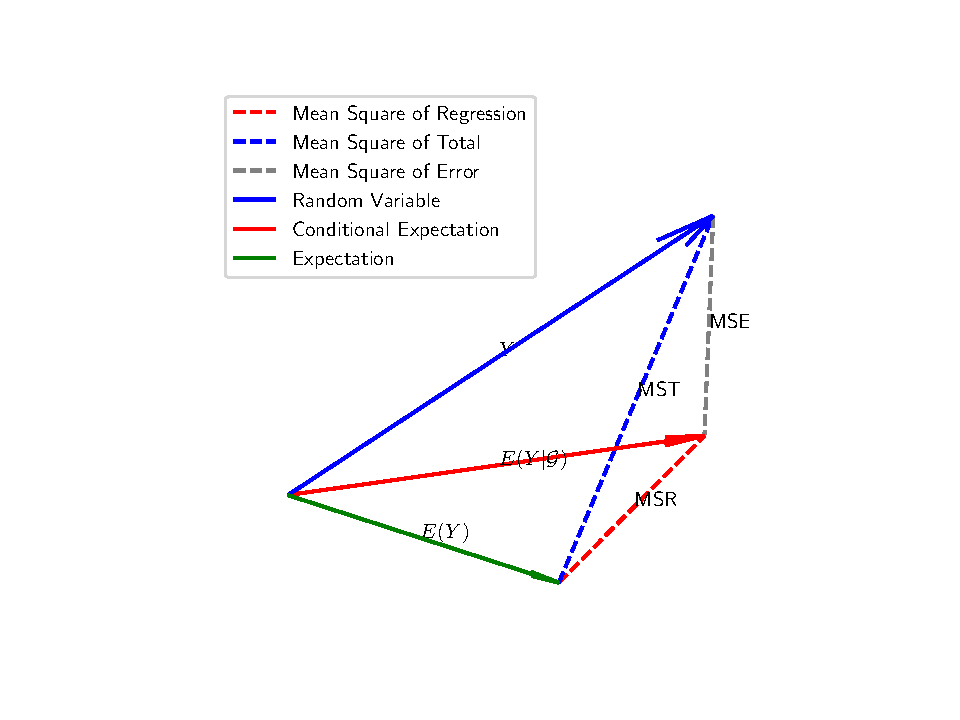
\includegraphics{figure/conditional.pdf}
	\vspace{-1.7cm}
	\caption{Conditional Expectation as a projection.}
	\label{fig:conditonalexpectation}
\end{figure}

The regression model can be structed as follows, suppose we have a random variable $Y$ defined on a probability space $(\Omega, \mathcal{F}, P)$, and a random map $X$ from $\Omega$ to a vector space $E$ (often denoted as $\R^p$). We can express $Y$ as the sum of its conditional expectation $E(Y|X)$ and the error term $Y-E(Y|X)$, which can be written as $m\circ X + \varepsilon$.

To estimate the conditional expectation from sample data, we need to minimize the empirical loss function:
$$
\argmin_{f \in \mathcal{H}} \frac{1}{n} \sum_{i=1}^n (y_i - f(x_i))^2,
$$

where $y_i$ is the value of $Y$ and $x_i$ is the value of $X$ in the $i$-th sample, and $\mathcal{H}$ is a suitable class of functions. The goal is to find a function $f$ that minimizes the difference between the predicted values and the actual values, as measured by the mean squared error.


There are many ways to optimize the empirical loss function. One of the simplest ways is to parameterize it. For instance, we can set the form of the hypothesis as follows:

There are various methods to optimize the empirical loss function. One of the simplest ways is to parameterize it. For example, we can define the form of the hypothesis as follows:
\begin{equation}
\mathcal{H} = \left\{f: \R^p \to \R, \quad x \mapsto c+ \beta^T x| \text{where}\ \beta \in \R^p, c \in \R \right\}.	
\end{equation}
In this case, the problem can be converted to:
$$
\argmin_{\beta \in \R^{p+1}} \frac{1}{n} \sum_{i=1}^n (y_i - \beta^T \tilde x_i)^2,
$$
where $\mathcal{H}$ is often referred to as the collection of affine functions, and the $\beta$ that minimize the square loss is
$$
\hat \beta = (X^T X)^{-1} X^T Y.
$$
The hypothesis space can also be represented as a reproducing kernel Hilbert space (RKHS). Assuming that $K: \R^p \times \R^p \to \R$ is a positive definite kernel function, there exists an inner product in $\mathcal{H}$ such that $K_x$ belongs to $\mathcal{H}$ for all $x\in \R^p$. According to the representer theorem \cite{scholkopf2001generalized}, there is a unique minimizer in the form of
$$
f = \sum_{i=1}^n \alpha_i K_{x_i}
$$
Moreover, the GLM can be utilized as a Hypothesis. In this scenario, $\mathcal{H}$ can be expressed as follows:
\begin{equation}
\mathcal{H} = \left\{f: \R^p \to \R, \quad x \mapsto g^{-1} \circ(c+ \beta^T x)| \text{where}\ \beta \in \R^p, c \in \R \right\},	
\end{equation}


Here, $g^{-1}$ refers to the inverse of the canonical link function and varies for different cases.


\begin{table}[htb]
\centering
\caption{The Canonical Link Function of GED.}
\vspace{.2cm}
\begin{tabular}{c c c}
\toprule
Distribution &Mean Function & Canonical Link Function \\
\midrule
$N(\mu,\sigma^2)$ & $b^\prime: \theta \mapsto \theta$ & $g: \mu \mapsto \mu$ \\
$Pois(\lambda)$ & $b^\prime: \theta \mapsto \E^{\theta}$& $g: \mu \mapsto \ln \mu$\\
$Bin(1,p)$ & $b^\prime: \theta \mapsto \frac{1}{1+\E^{-\theta}}$ & $g: \mu \mapsto \ln \frac{\mu}{1-\mu}$ \\
\bottomrule
\end{tabular} 
\label{tab:GLM}
\end{table}















